\section{Implementation}

We implemented our system as a web application. The client-side program is
completely written in HTML/JavaScript and is compatible with most modern web
browsers, and the server is written in the Go programming language (most notably
the Go {\tt http} package~\cite{gohttp} to implement most of the front-end
server functionality). We also used {\tt socket.io}~\cite{socketio}, a full-duplex
real-time communication framework using the {\tt websocket}
technology~\cite{websock}, instead of standalone HTTP requests/responses for a
more streamlined design. Open-source {\tt socket.io} libraries for
JavaScript~\cite{jssocketio} and Go~\cite{gosocketio} are the only external
libraries we used to implement our OT framework. We also used a JavaScript code
snippet from Internet~\cite{linenumber} to improve the look of our user
interface. All source code of the project is publicly available at
\url{https://github.com/huangyihe/etherpad-paxos}.

\subsection{Client-side Script}

A JavaScript program implements all logic and functionality described in
Section~\ref{sec:design_client}. The program generates client operations by
listening on key strokes. Generated operations (which are JavaScript objects)
are converted to JSONs~\cite{json} before being transmitted over the network via
{\tt socket.io}. The client-side program contains 473 lines of code, excluding
all external libraries and code snippets.

\subsection{Server-side Paxos Integration}

\begin{figure}[t!]
  \centering
  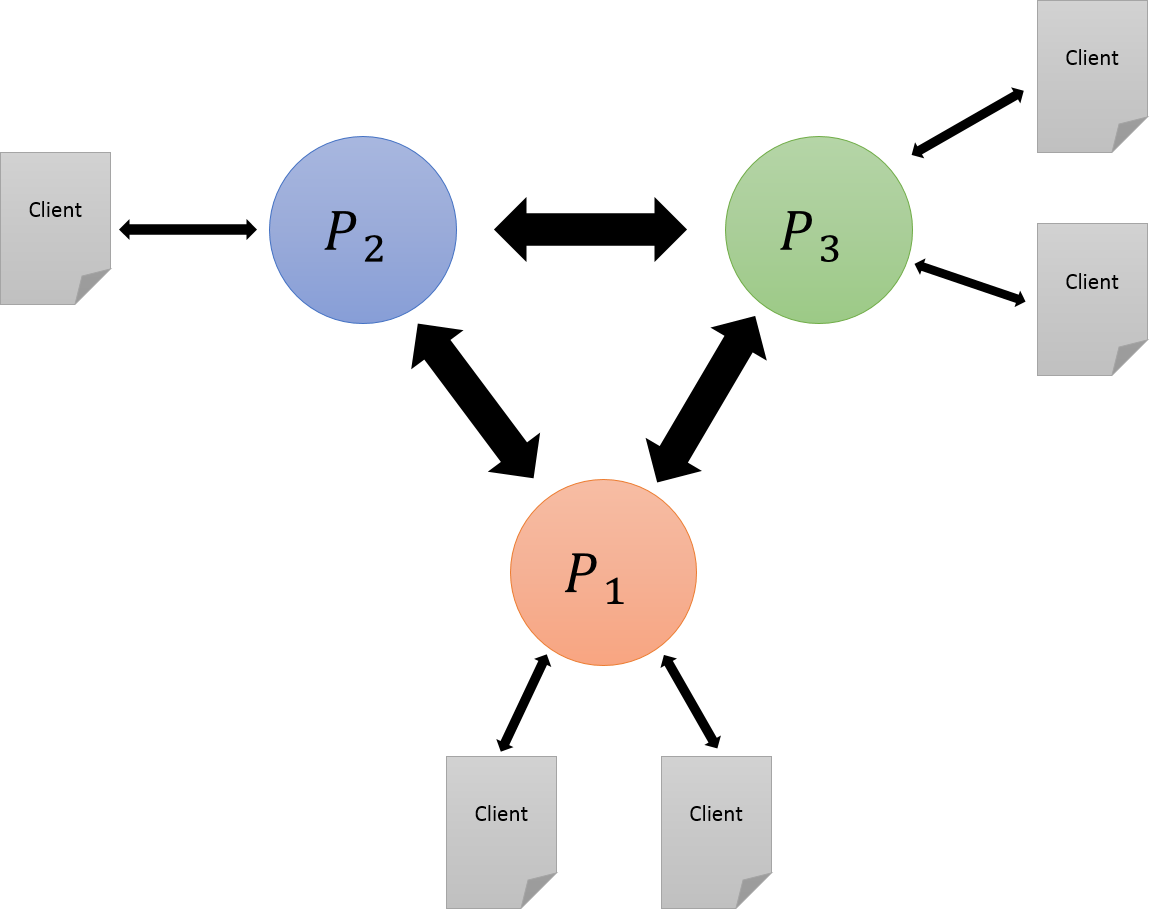
\includegraphics[width=0.45\textwidth]{system_overview.png}

  \caption{High-level overview of the implemented system. $P_1$, $P_2$, $P_3$
  are replicated servers talking to each other using Paxos (a three-server
  configuration shown here), and clients are connected to each other via these
  servers. Clients can connect to different Paxos peers.}
  
  \label{fig:system}
\end{figure}

To improve availability of the server, we replicate the server using the Paxos
protocol~\cite{lamport1998part}. Clients can connect to any server in the Paxos
quorum without noticing the difference. One challenge to address is to make sure
that clients connected to different Paxos peers can see each other's updates in
a timely manner. We achieve this by running a background thread at each Paxos
server (called the ``auto-apply'' thread) whose sole job is to periodically look
for new decided entries in the Paxos log and apply them if any.
Figure~\ref{fig:system} gives a high-level overview of the system.

The Go program contains 630 lines of code, excluding Paxos\footnote{There are
minor modifications to the Paxos library, though.} and external libraries.
